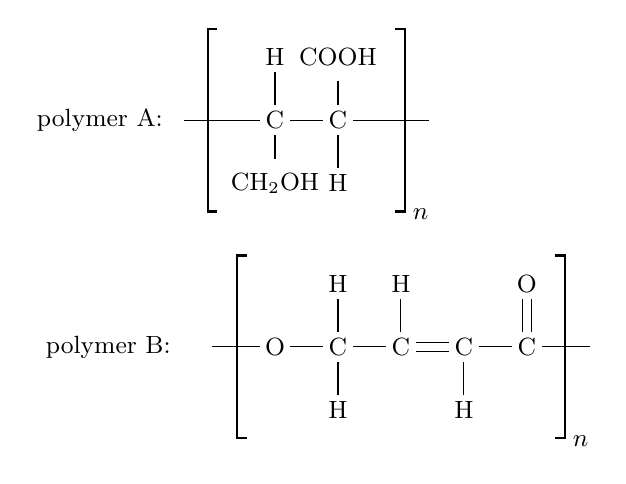
\begin{tikzpicture}
\draw (-1.150,0.000) -- (-0.192,0.000);
\draw (0.192,0.000) -- (0.608,0.000);
\draw (0.992,0.000) -- (1.950,0.000);
\draw (0.000,0.192) -- (0.000,0.608);
\draw (0.800,0.192) -- (0.800,0.493);
\draw (0.000,-0.192) -- (0.000,-0.493);
\draw (0.800,-0.192) -- (0.800,-0.608);
\node[inner sep=0pt,font=\small] at (0.000,0.000) {C};
\node[inner sep=0pt,font=\small] at (0.800,0.000) {C};
\node[inner sep=0pt,font=\small] at (0.000,0.800) {H};
\node[inner sep=0pt,font=\small] at (0.800,-0.800) {H};
\node[inner sep=0pt,font=\small] at (0.000,-0.800) {$\mathrm{CH_2OH}$};
\node[inner sep=0pt,font=\small] at (0.800,0.800) {$\mathrm{COOH}$};
\draw[thick] (-0.730,1.160) -- (-0.850,1.160) -- (-0.850,-1.160) -- (-0.730,-1.160);
\draw[thick] (1.530,1.160) -- (1.650,1.160) -- (1.650,-1.160) -- (1.530,-1.160);
\node[font=\small] at (1.850,-1.200) {$n$};
\node[anchor=east,font=\small] at (-1.300,0) {polymer A:};
\draw (-0.800,-2.880) -- (-0.192,-2.880);
\draw (0.192,-2.880) -- (0.608,-2.880);
\draw (0.800,-2.688) -- (0.800,-2.272);
\draw (0.800,-3.072) -- (0.800,-3.488);
\draw (0.992,-2.880) -- (1.408,-2.880);
\draw (1.600,-2.688) -- (1.600,-2.272);
\draw (1.792,-2.820) -- (2.208,-2.820);
\draw (1.792,-2.940) -- (2.208,-2.940);
\draw (2.400,-3.072) -- (2.400,-3.488);
\draw (2.592,-2.880) -- (3.008,-2.880);
\draw (3.140,-2.688) -- (3.140,-2.272);
\draw (3.260,-2.688) -- (3.260,-2.272);
\draw (3.392,-2.880) -- (4.000,-2.880);
\node[inner sep=0pt,font=\small] at (0.000,-2.880) {O};
\node[inner sep=0pt,font=\small] at (0.800,-2.880) {C};
\node[inner sep=0pt,font=\small] at (0.800,-2.080) {H};
\node[inner sep=0pt,font=\small] at (0.800,-3.680) {H};
\node[inner sep=0pt,font=\small] at (1.600,-2.880) {C};
\node[inner sep=0pt,font=\small] at (1.600,-2.080) {H};
\node[inner sep=0pt,font=\small] at (2.400,-2.880) {C};
\node[inner sep=0pt,font=\small] at (2.400,-3.680) {H};
\node[inner sep=0pt,font=\small] at (3.200,-2.880) {C};
\node[inner sep=0pt,font=\small] at (3.200,-2.080) {O};
\draw[thick] (-0.360,-1.720) -- (-0.480,-1.720) -- (-0.480,-4.040) -- (-0.360,-4.040);
\draw[thick] (3.560,-1.720) -- (3.680,-1.720) -- (3.680,-4.040) -- (3.560,-4.040);
\node[font=\small] at (3.880,-4.080) {$n$};
\node[anchor=east,font=\small] at (-1.200,-2.880) {polymer B:};
\end{tikzpicture}
